% !TEX root = recommending-interesting-writing.tex
\section{Evaluation}
\label{sec:experiments}

We study the performance of \acrlong{rfs} on a dataset that we collect to assess whether \gls{rfs}, in addition to providing interpretable recommendations to help editors make decisions about articles.

\paragraph{Data Collection and Preprocessing.} For positive examples, we use the historical set of articles curated by editors at The Browser. We augment the training data with articles selected by the editors of other curation services, and treat all positively-labeled examples curated by editors as data from a single user due to a paucity of data. We use articles from news websites as examples with negative labels, and collect additional articles with negative labels from websites most-featured by the editors to mimic the editorial process of reading a large swath of articles in a feed and distilling an article list to a select few. For preprocessing the data we use the tokenizer released by \citet{devlin2019bert:} and discard words not recognized by the tokenizer. This procedure leaves a dictionary with $30$k words, and $148$k training examples with $28$k positive labels.

\paragraph{Metrics} Performance of the recommendation models is assessed with recall, and $15\%$ of the data is held-out for validation and test sets.

\paragraph{Experimental setup: RankFromSets} The performance of the model was similar for large embedding sizes, and we selected the dimension of the embeddings to be $25$. We cross-validate using the RMSProp optimizer~\citep{tieleman2012lecture} and grid search over learning rates of $\{10^{-1}, 10^{-3}, 10^{-4}, 10^{-5}\}$ and select the best-performing model for deployment.

\paragraph{Experimental setup: BERT}

for rankfromsets we searched over 6 embedding sizes [10,25,50, 100, 500, 1000] and 5 batch sizes [500, 1000, 2000, 5000, 10000]. We tried two optimizers, RMS and SGD, both with a momentum of 0.9 and learning rates of [1e-2, 1e-3, 1e-4, 1e-5] for RMS, while learning rates for SGD varied based on batch size and average token count
Breakdown of Data: Train -      Total: 100797            Positive: 18598                 Negative: 82199
Test -      Total: 272448          Positive: 4049                  Negative: 268399
Evaluation -      Total: 272447            Positive: 4039                  Negative: 268348
Both models used the same randomly selected 50k articles from the evaluation set for validation, and the entire test set was used at the end to generate predictions on new data.

for BERT, used AdamW optimizer with a linear scheduler, with 4 different learning rates [2e-5, 3e-5, 4e-5, 5e-5] and a batch size of 32. Tried four different amounts for warmup steps [100, 1000, 1000, 10000] and total training steps were within the set [500, 5000, 50000, 100000] depending on the warmup step amount
First 510 tokens were taken from the article to generate predictions so as to fit the BERT length requirements

\begin{figure}[!tb]
  \centering
  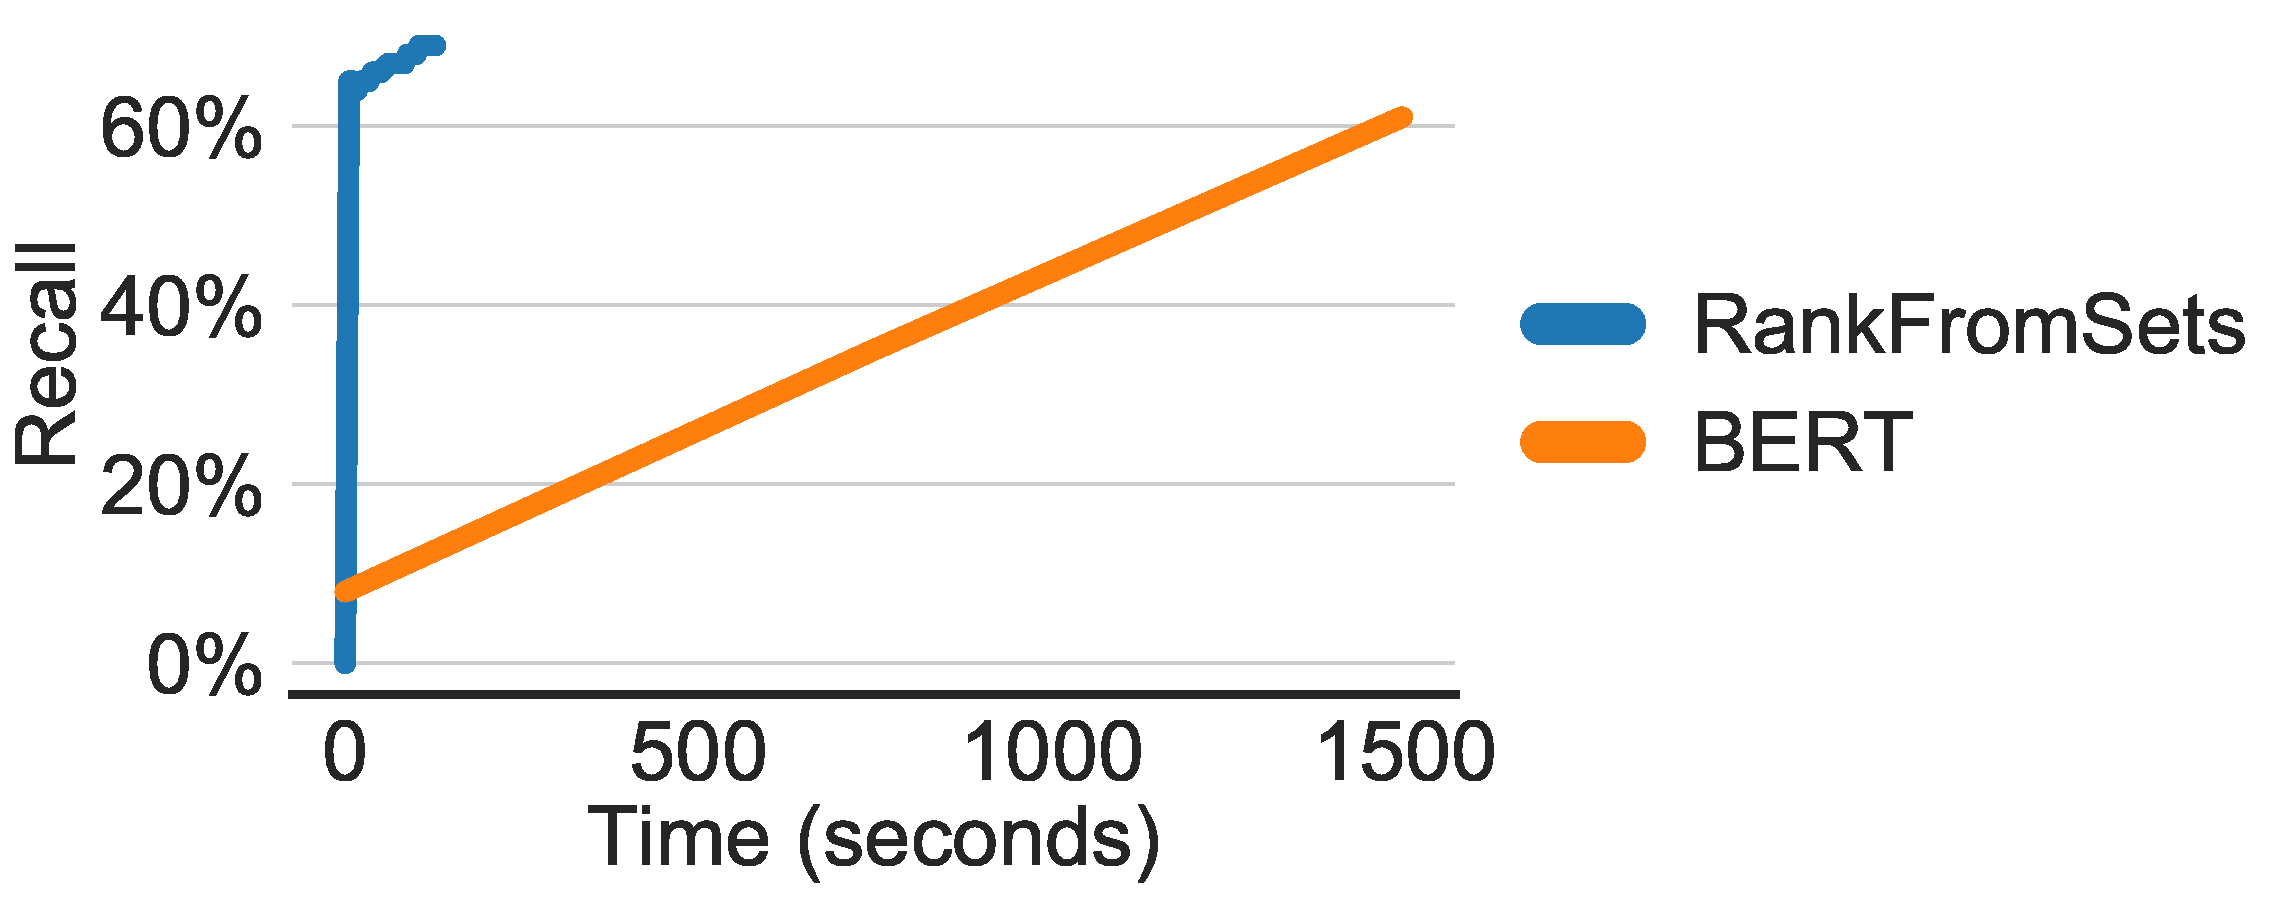
\includegraphics[width=0.95\linewidth]{fig/training-recall}
  \caption{\acrlong{rfs} outperforms models based on word embeddings
    permutation-marginalized recurrent neural networks (denoted by LSTM) on meal
    recommendation. The recommendation models are trained on data from a food
    tracking app as described in \Cref{sec:experiments_meals} and are evaluated
    using the sampled recall metric, \Cref{eq:sampled-recall}. The inner
    product, neural network, and residual regression functions for \acrlong{rfs}
    are in \Cref{eqn:rankfromsets,eqn:neural-network,eqn:residual}.}
  \label{fig:training-recall}
\end{figure}
% !TEX root = ../recommending-interesting-writing.tex
\begin{table}[tb]
\centering
\begin{tabular}{lSS}
\toprule
Recommendation Model & \multicolumn{1}{c}{Recall @ 1000 (\%)}
\\
\midrule
\acrlong{rfs} &  \bfseries 53.1\\
\acrshort{bert} & 46.6 \\
\bottomrule
\end{tabular}
% BERT 466/1000
% rankfromsets 531/1000
% \vspace{1ex}
\caption{\gls{rfs} outperforms \acrshort{bert} in an offline evaluation, on a task of predicting which articles editors at The Browser would feature based on words in the articles.}
\label{tab:recall}
\end{table}

BERT 466/1000
rankfromsets 531/1000

\paragraph{Evaluation.} Qualitatively, editors at The Browser preferred the recommendations of our pipeline over their current workflow of a reading list sorted in terms of recency and use the system in production.